\documentclass[fleqn,10pt]{olplainarticle}
\usepackage{hyperref}

\usepackage{xcolor}
\hypersetup{
	colorlinks,
	linkcolor={red!50!black},
	citecolor={blue!50!black},
	urlcolor={blue!80!black}
}

\usepackage{enumitem}

\usepackage{float}

\usepackage{caption}
\usepackage{subcaption}
\usepackage{multicol}

% Use option lineno for line numbers 

\title{Strengthening Cryptobridges: Assessing Hashing Accuracy in Ethereum with a Focus on Merkle Patricia Trie}

\author[1]{jistro.eth and ariutokintumi.eth}
%\author[2]{Ariutokintumi.eth }
%\affil[1]{Address of first author}
%\affil[2]{Address of second author}

\keywords{Merkle tree, PATRICIA Trie, Ethereum, Blockchain}


\begin{abstract}
This document explores Merkle Trees, Ethereum block structures, transaction data, and the implementation of Merkle Patricia Tries, emphasizing successful pre-merge verification but noting challenges in post-merge scenarios.
\end{abstract}

\begin{document}

\flushbottom
\maketitle
\thispagestyle{empty}

\tableofcontents

\section{Merkle tree}

Before delving into the topic, it is important to understand the concept of a Merkle Tree. A Merkle Tree is a binary tree of hash values where each leaf node represents a single piece of data or the hash of a piece of data. It is commonly employed to efficiently verify the integrity of large datasets. Invented by Ralph Merkle in 1979, it is an integral part of all blockchains. \cite{kumar_introMerkleTree_2023}

The most common hashing algorithm in a Merkle tree is SHA-256 (Secure Hash Algorithm 256), which is part of the SHA-2 algorithm family, producing a fixed-length, 256-bit (32-byte) hash value. The key features of SHA-256 are \cite{gitlan_whatSHA256_2023}:

\begin{itemize}
	\item \textbf{Message Length}: The length of the readable text before it is encrypted should be less than 264 bits.
	\item \textbf{Digest Length}: The hash digest length should be 256 bits.
	\item \textbf{Irreversibility}: All SHA-256 outputs are irreversible by design. For each input, you have exactly one output, but not the other way around. Multiple inputs produce the same output. The output has a fixed size, but the input doesn’t have size restrictions.
\end{itemize}

As seen in Figure \ref{fig:merkletree}, the tree has three parts: Leaves, Nodes/Branches, and a Root. For the use of every leaf, it represents a transaction. This gives us the transactions hashed to later concatenate with another hash. This process is done 
\(n\) number of times until we get the Merkle root.

\begin{figure}[H]
	\centering
	\includegraphics[width=0.8\linewidth]{"./img/MerkleTree"}
	\caption{lustration of Merkle Tree}
	\label{fig:merkletree}
\end{figure}

To verify if a transaction really happened in a block (as illustrated in Figure \ref{fig:merkletree}), for example, Transaction 1, we only need to verify with \(H_{1+2}\), and by combining \(H_{[n-1]+n}\) we get the Merkle root. If some data is not correlated with the hash, the root will be different than the result. This is what we call a Merkle proof. However, not only can we prove a leaf, but we can also prove a node or even the root itself.



\section{The Ethereum Block}

The structure of an Ethereum (ETH) block undergoes a change in ''The Merge.'' As the name implies, ''The Merge'' involves combining the old blocks (execution layer) with the new Beacon Chain blocks (consensus layer), which operates on Proof of Stake (PoS)   

Under PoS, an Ethereum block is comprised of three main parts \cite{kirshner_ethereumBlock_2023}:

\subsection{Administration}

Is the the metadata of the block

\begin{itemize}[noitemsep]
	\item \texttt{slot}: The position of the block in the beacon chain blockchain (eg the 100,000 block is in slot 100000)
	\item \texttt{proposer\_index}: The proposer who created this block
	\item \texttt{parent\_root}: The root hash of a Merkle tree of the previous block
	\item \texttt{state\_root}: The root hash of a Merkle tree which stores the state of the Beacon Chain (BeaconState)
	\item \texttt{randao\_reveal}: Protocol-verified randomness, generated between all block proposers during an epoch. Randomness is critical to the Beacon Chain; security depends on being able to unpredictably and uniformly select block proposers and committee members.
	\item \texttt{graffiti}: An optional 32-byte field in which block proposers can put anything they want. Often used by mining pools to log their blocks.
	\item \texttt{signature}: The signature the block proposer creates to take responsibility (add to blockchain and collect reward if good, get slashed if bad). Created by combining the BeaconState, BeaconBlock and the proposer's private key.
\end{itemize}

\subsection{Consensus}

Is the layer coordinating the Beacon Chain providing the cryptographic security of PoS

\begin{itemize}[noitemsep]
	\item \texttt{deposit\_root}: The root hash of a Merkle tree which stores the ETH deposits into the staking contract (required to become a validator)
	\item \texttt{deposit\_count}: Amount of ETH in the staking contract
	\item \texttt{block\_hash}: Hash of the block
	\item \texttt{deposits}: Amount of validator deposits which have been included in this block by the block proposer. Interestingly, the only non-0 value I could find was in the genesis block
	\item \texttt{voluntary\_exits}: Withdrawals from the staking contract
	\item \texttt{attestations}: A list of all the signatures that attested to this block. Ethereum PoS elects a proposer who is charged with building (or selecting) a block and proposing it to the network. Attesters review the block and, if it's valid, sign it with their keys.
	\item \texttt{proposer\_slashings}, \texttt{attester\_slashings}: Validators that have performed a hostile action against the network. The network confiscates a portion of their staked ETH and ejects them from the validator set.
	\item \texttt{sync\_aggregate}: Contains the aggregate BLS signature for the active sync committee. A sync committee is a group of 512 validators, randomly assigned once every 256 epochs (approximately 27 hours). This committee creates the signatures needed for an efficient light client.
	\item \texttt{sync\_committee\_bits} An efficient representation of committee participation.
	\item \texttt{sync\_committee\_signature}: The signature the sync committee creates to take responsibility for the block/epoch.
	
\end{itemize}

\subsection{Execution}

Is the data of the block, (almost) exactly mirroring PoW blocks.

\begin{itemize}[noitemsep]
	\item \texttt{baseFeePerGas}: Building on EIP-1559, the proposal establishes a minimum cost, known as the base fee, for each unit of gas in Ethereum transactions. This base fee is entirely burned with every block creation, and its value adjusts based on the fullness of the preceding block, allowing for a maximum change of 12.5\% per block. Additionally, EIP-1559 introduces the concept of difficulty, which approximates the time a miner should spend calculating a hash function before discovering a block. 
	\begin{math}
		\frac{Network~hash~rate} {difficulty} = average~block~time
	\end{math}
	It's important to note that these dynamics are no longer applicable under Proof of Stake, signaling a broader shift in the Ethereum consensus mechanism \cite{buterin_eip1559_2019}.
	
	\item \texttt{extraData}: An (optional) 32-byte field in which block proposers can put anything they want. Often used by mining pools to log their blocks.
	Similar to the graffiti in the consensus layer
	\item \texttt{gasLimit}: Total gas available to the block
	\item \texttt{gasUsed}: Gas used by the block
	\item \texttt{hash}: Hash of the block
	\item \texttt{logsBloom}: A Bloom filter is a probabilistic structure that allows a user to filter through each element in the block.
	minimizes the number of queries a client needs to make.
	\item \texttt{Miner}: The Ethereum address of the miner who successfully created this block
	\item \texttt{mixHash}: Intermediate value calculated from nonce, used for validation
	\item \texttt{nonce}: Extra data miners add to a block before hashing. A block is created when this hash matches a specific value; mining is the process of attempting to find this value by altering the nonce.
	\item \texttt{number}: Ethereum block number. Similar to slot in the consensus layer
	\item \texttt{parentHash}: The root hash of a Merkle tree of the previous block
	\item \texttt{receiptsRoot}: The root hash of a Merkle tree which stores the receipts created by the transactions in a block. A receipt includes: block number, block hash, associated contracts, gas used, the stateRoot at the time (before) transaction, etc.
	\item \texttt{size}: Size of the block in bytes
	\item \texttt{stateRoot}: The root hash of a Merkle tree which stores the entire state of the Ethereum Virtual Machine (EVM), account balances, contract storage, contract code, etc
	\item \texttt{timestamp} the date/time when the block was created, as reported by the block proposer
	\item \texttt{totalDifficulty}: The cumulative value of the difficult required to build the chain up until this block
	No longer applicable under Proof of Stake
	\item \texttt{transactionsRoot}: The root hash of a Merkle tree which stores the transactions contained within the block.
	\item \texttt{transactions}: An ordered list of all the transactions executed within the block.
\end{itemize}

\subsection{Transaction data}

Inside \texttt{transactions} written in blocks there are three main sections \cite{kirshner_ethereumTx_2023}:

\subsubsection{Metadata}

The metadata details of a transaction 

\begin{itemize}[noitemsep]
	\item \texttt{blockHash}: The unique signature created by hashing the block the transaction is contained in.
	\item \texttt{blockNumber}: A unique, sequential number that identifies the block's position in the blockchain.
	\item \texttt{chainId}: Applying EIP-155 for simple replay attack protection, this field signifies whether the transaction is on the Ethereum chain or other EVM-compatible chains \cite{buterin_eip155_2016}.
	\item \texttt{from}: Address (wallet or smart contract) the transaction is being sent from
	\item \texttt{gas}: Units of gas used by the transaction
	\item \texttt{gasPrice}: Amount paid (in WEI) per unit of gas for this transaction
	\item \texttt{hash}: Hash of the transaction
	\item \texttt{maxFeePerGas}: Maximum amount (WEI per gas) the user who created the transaction is willing to pay. Inclusive of base fee and priority fee
	\item \texttt{maxPriorityFeePerGas}: Maximum amount (WEI per gas) above the base fee the user who created the transaction is willing to pay. This fee will be paid directly to the miner/validator as a tip to incentive inclusion.
	\item \texttt{nonce}: Number of transactions sent from a given address. Once imprinted on a block, the wallet's nonce is increased. Protects against replay attacks
	\item \texttt{r, s, v}: Three values that form the signature of the user who created the transaction. They can be used to verify that the user authorized the transaction before it was executed in the EVM.
	\item \texttt{to}: Address (wallet or smart contract) the transaction is being sent to
	\item \texttt{transactionIndex}: Position of transaction within block
	\item \texttt{type}: There are two types: a new contract (0x0) and all others (0x2).
	\item \texttt{value}: Amount of ETH being transferred.
\end{itemize}

\subsubsection{Cache}

This section pertains to the \textbf{\texttt{accessList}}, which comprises a list of addresses and keys that the transaction expects to utilize. While the transaction retains the ability to utilize resources outside this list, it incurs a higher gas cost.

The introduction of the \texttt{accessList} was facilitated by EIP-2929, allowing clients to fetch and cache data for use during the transaction.

EIP-2929 brought about several key changes, including increased gas costs for state access opcodes, the introduction of \texttt{accessed\_addresses} and \texttt{accessed\_storage\_keys} sets, and the concept of the \texttt{AccessList}. These changes collectively address historical issues related to opcode underpricing and potential attack vectors \cite{buterin_eip2929_2020}. Following EIP-2929, EIP-2930 was introduced, adding a new transaction type that includes an access list, a list of addresses and storage keys that the transaction plans to access. While accesses outside this list remain possible, they incur higher costs \cite{buterin_eip2930_2020}.

As of now, there is approximately a 10\% discount for using addresses and keys in the \texttt{AccessList}. However, it's crucial to note that this discount may increase in the future as Ethereum evolves to support light clients.



\subsubsection{Data}

This section delves into the transaction payload, encompassing either smart contract code or an API call. The data payload transmitted by the transaction serves diverse purposes and can be harnessed in three distinct ways:
\begin{enumerate}
	\item ETH transfer: Nill payload (\texttt{0x00}).
	\item Smart contract API call: Contains the name of the function and its parameters.
	\item New smart contract: Includes the code of the smart contract.
\end{enumerate}

While the data in the input field is recorded in binary (Figure \ref{fig:newsc}), it can be translated back into a human-readable form (Figure \ref{fig:scapicall}).

\begin{figure}
	\begin{subfigure}{.5\textwidth}
		\centering
		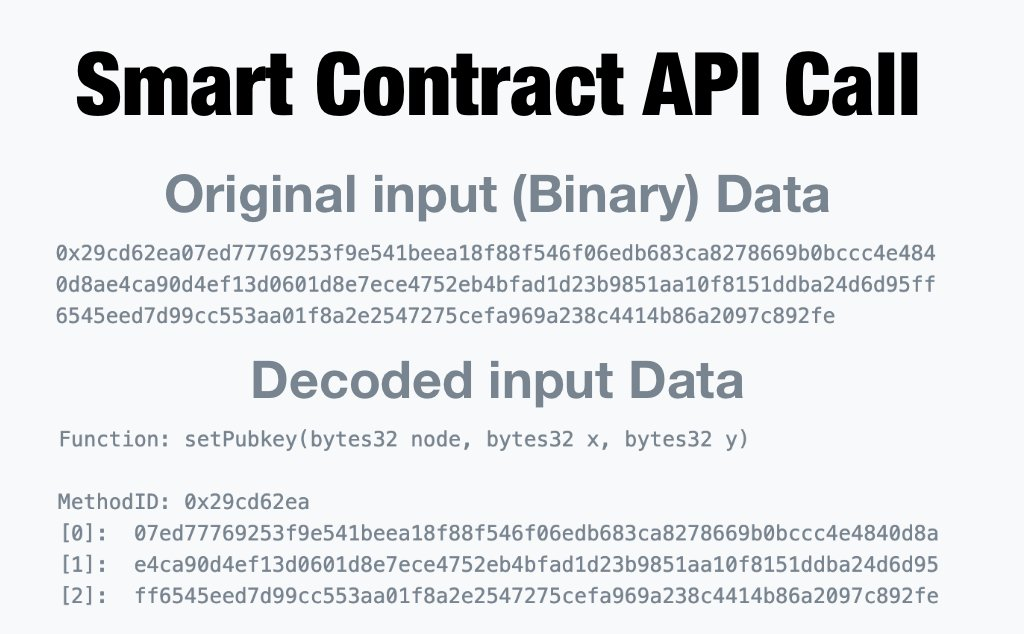
\includegraphics[width=0.8\linewidth]{img/scAPICall}
		\caption{Input data in binary}
		\label{fig:scapicall}
	\end{subfigure}
	\begin{subfigure}{.5\textwidth}
		\centering
		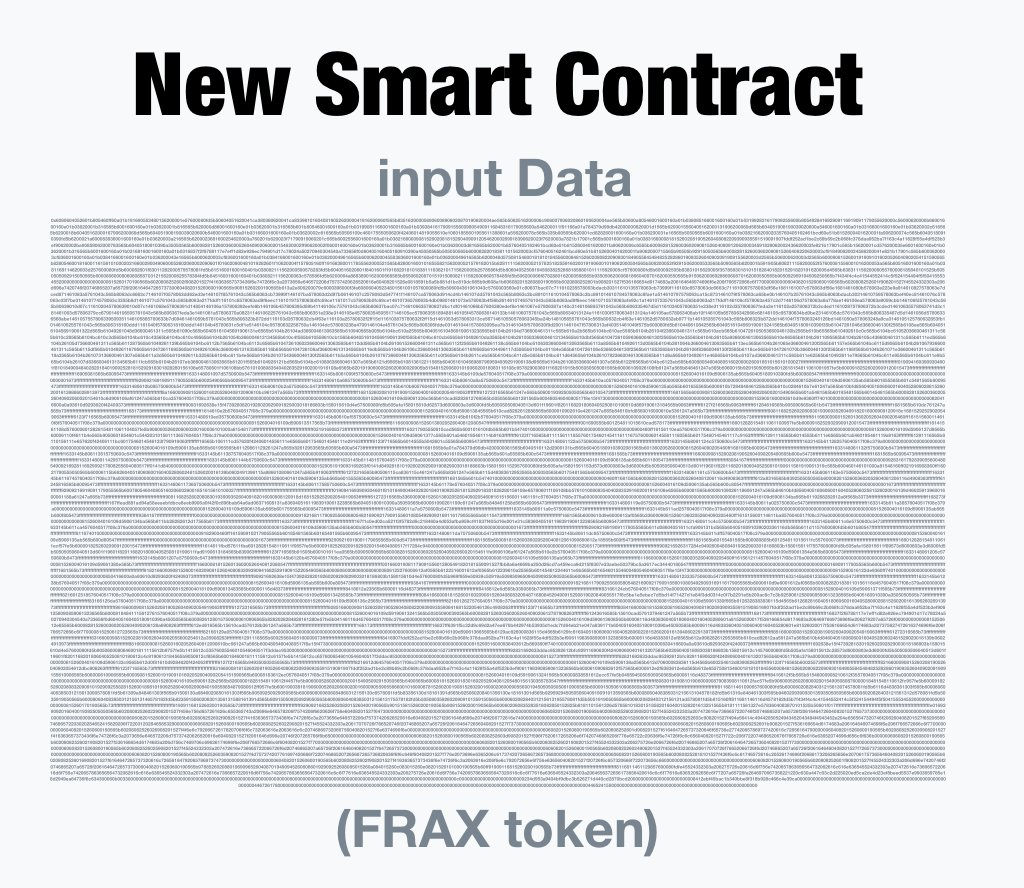
\includegraphics[width=0.8\linewidth]{img/NewSC}
		\caption{Input data in human-readable form }
		\label{fig:newsc}
	\end{subfigure}
	\caption{Input data \cite{kirshner_ethereumTx_2023}}
	\label{fig:inputIMG}
\end{figure}

It's crucial to note that the input field exists on-chain but is not part of the EVM state. Instead, it provides data for the contract to use during the transaction and is not tracked by Ethereum or used in consensus.

The EVM can only utilize the data supplied in that specific transaction; it does not have the ability to look back.

This property proves particularly useful for applications aiming to write historical data to the Ethereum blockchain (e.g., for manual retrieval later) but do not necessitate direct EVM access.

\section{Development}

\subsection{Merkle tree implementation}

In the development process, we leverage acquired knowledge to construct the \texttt{blockHash} utilizing Merkle trees and Ethereum node providers in the prescribed order for accurate hashing \cite{anuragp_answer_2019}. The sequence of elements used includes:

\begin{multicols}{3}
\begin{enumerate}[noitemsep]
	\item \texttt{parentHash}
	\item \texttt{sha3Uncles}
	\item \texttt{miner}
	\item \texttt{stateRoot}
	\item \texttt{transactionsRoot}
	\item \texttt{receiptsRoot}
	\item \texttt{logsBloom}
	\item \texttt{difficulty}
	\item \texttt{number}
	\item \texttt{gasLimit}
	\item \texttt{gasUsed}
	\item \texttt{timestamp}
	\item \texttt{extraData}
	\item \texttt{mixHash}
	\item \texttt{nonce}
\end{enumerate}
\end{multicols}
Despite employing this approach to gather block information, it has been determined that this method does not yield the correct \texttt{blockHash}. This is because Ethereum uses another type of tree structure, namely a \textbf{Merkle Patricia Tree}. This tree is a combination of a Merkle tree and a Patricia Trie.


\subsection{PATRICIA Trie}

Developed by Donald R. Morrison and published in October 1968, a Practical Algorithm to Retrieve Information Coded in Alphanumeric (PATRICIA) Trie is a special case of Radix Trie that follows three defined rules \cite{osiek_patricia_2020,eisler_trie_2013}:

\begin{itemize}[noitemsep]
	\item Each node has two children, and all internal nodes of the tree have at least one child.
	\item A node is only split into a prefix with two children (each child forming a branch) if two words share the same prefix.
	\item Every word ending will be represented with a value within the node different than null.
\end{itemize}

Let's see a simple and graphical example based on the David Eisler video \cite{eisler_trie_2013}:

We have this list of text in this order:

\begin{multicols}{4}
	\begin{enumerate}[noitemsep]
		\item ROMANE
		\item ROMANUS
		\item ROMULUS
		\item RUBENS
		\item RUBER
		\item RUBICON
		\item RUBICONDUS
		\item RUB
	\end{enumerate}
\end{multicols}

First, with ''ROMANE,'' we group the characters into a single edge. In this case, we put the null terminator on the edge to indicate that it's a complete word. Next, we add ''ROMANUS.'' Since ''ROMAN'' is common between both words, we branch off with ''US,'' and the null terminator in the ''E'' with a null. Continuing the same process, we add ''RUB.'' As seen in Figure \ref{fig:PatriciaTrieAdd}, ''RUB'' has all the branches in common, so it is already in the tree. We add an edge with a null terminator to label ''RUB'' as a word.


\begin{figure}[h]
	\centering
	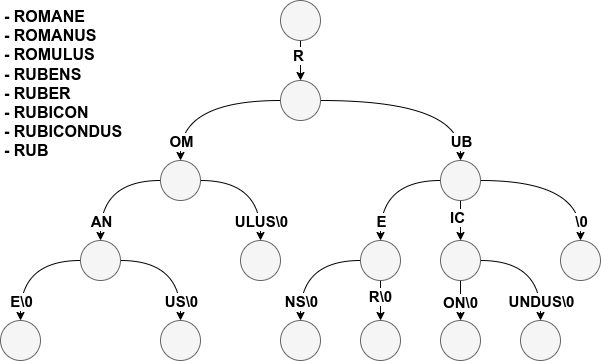
\includegraphics[width=0.8\linewidth]{img/PATRICIA-TrieAdd}
	\caption{Patricia trie tree example from \cite{eisler_trie_2013}}
	\label{fig:PatriciaTrieAdd}
\end{figure}

\subsection{Merkle PATRICIA Trie}

Merkle Patricia Trie (MPT) serves as a fundamental data structure within the Ethereum network, specifically designed for efficient state storage and retrieval. Much like the Merkle tree, every node in the MPT obtains a hash value through the sha3 hash of its contents. It's important to note that the keys and values stored in the MPT do not directly mirror the key-value pairs of the Ethereum state. Instead, the value stored in the storage represents the content of the MPT node, with the key being the hash of this particular node.

Key-values of the Ethereum state are represented as paths on the MPT, and nibbles are used as the unit to distinguish key values. Each node in the MPT can have up to 16 branches, with a branch node being an array of 17 items composed of 1 node value and 16 branches.

A node without a child is termed a leaf node, comprising two essential elements: its path and value. For instance, in the scenario outlined by Kim \cite{kim_Ethereum_MPT_2018}, if the key \texttt{0xBEA} contains 1000 and the key \texttt{0xBEE} contains 2000, a branch node with the \texttt{0xBE} path would be created. Underneath this node, two leaf nodes with paths \texttt{0xA} and \texttt{0xE} would be attached.

\begin{figure}[H]
	\centering
	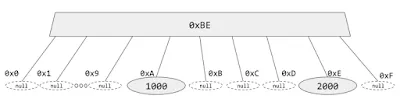
\includegraphics[width=0.7\linewidth]{img/MPT_E1}
	\caption{Example of MPT from  \cite{kim_Ethereum_MPT_2018}}
	\label{fig:mpte1}
\end{figure}

The MPT encompasses three node types: leaf nodes, branch nodes, and extension nodes. A leaf node, consisting of a path and value, contrasts with a branch node, which manifests as an array of items. Extension nodes, serving as optimized nodes, compress branch nodes containing only one child. To distinguish between leaf and extension nodes, the MPT introduces a prefix to the path. For even-numbered nibbles in leaf nodes, \texttt{0x20} is added, while odd-numbered nibbles receive \texttt{0x3}. In extension nodes, \texttt{0x00} is appended for even-numbered nibbles, and \texttt{0x1} for odd-numbered nibbles, ensuring consistent byte representation of paths \cite{kim_Ethereum_MPT_2018}.

\begin{figure}[h]
	\centering
	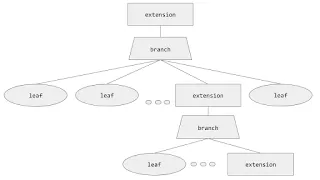
\includegraphics[width=0.7\linewidth]{img/MPT_E2}
	\caption{Structure of MPT from  \cite{kim_Ethereum_MPT_2018}}
	\label{fig:mpte2}
\end{figure}

\subsection{Merkle PATRICIA Trie implementation}

Upon employing the correct implementation using in the examples from Gabriel Rocheleau \cite{rocheleau_ethereums_2022} with the JavaScript library \texttt{ethereumjs/rlp} and \texttt{ethereum-cryptography/keccak}, we have successfully verified the accuracy of transaction and block hashes pre-merge. In this illustration, we utilized a legacy Ethereum transaction with the hash \\ \texttt{0x39fbe5446a0be5cbf62c2b623b33bc3a93cf9ec04439218c45b5eafdea736de2}. For the block reference, we chose block \texttt{400000}. The results, as depicted in Figure \ref{fig:hashpremerge}, confirm the correctness of the hashing process.

\begin{figure}[h]
	\centering
	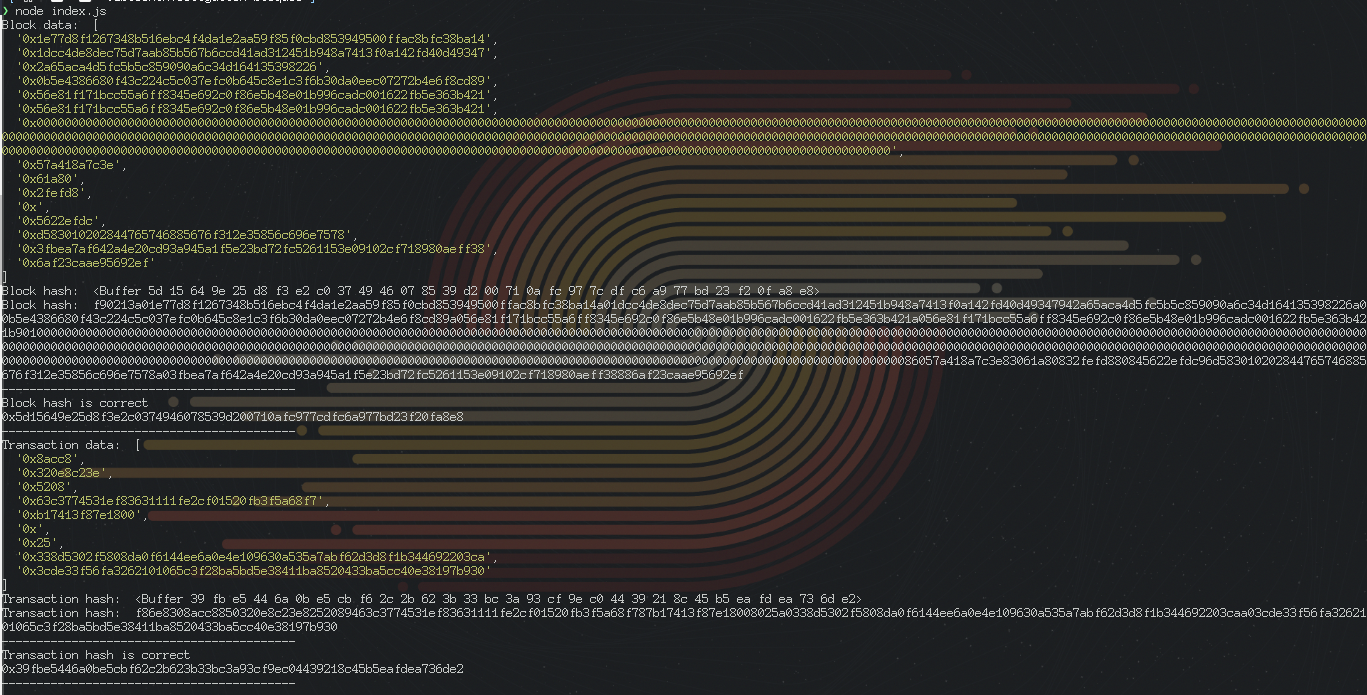
\includegraphics[width=1\linewidth]{img/HashPreMerge}
	\caption{Output of the hashing process using pre-merge data}
	\label{fig:hashpremerge}
\end{figure}


However, it's noteworthy that using transactions post-merge, such as smart contract creations or interactions, and post-merge blocks provides an improper output. For example, we utilized the transaction hash \texttt{0x36855e78a4056dee5eee89ab8b56e89df27135195d23ed96b532f8bb8db99e78}, which corresponds to a type 2 transaction (interaction with a smart contract), and the block containing that transaction (\texttt{18903867}) as seen in Figure \ref{fig:hashpostmergeerror}

\begin{figure}[h]
	\centering
	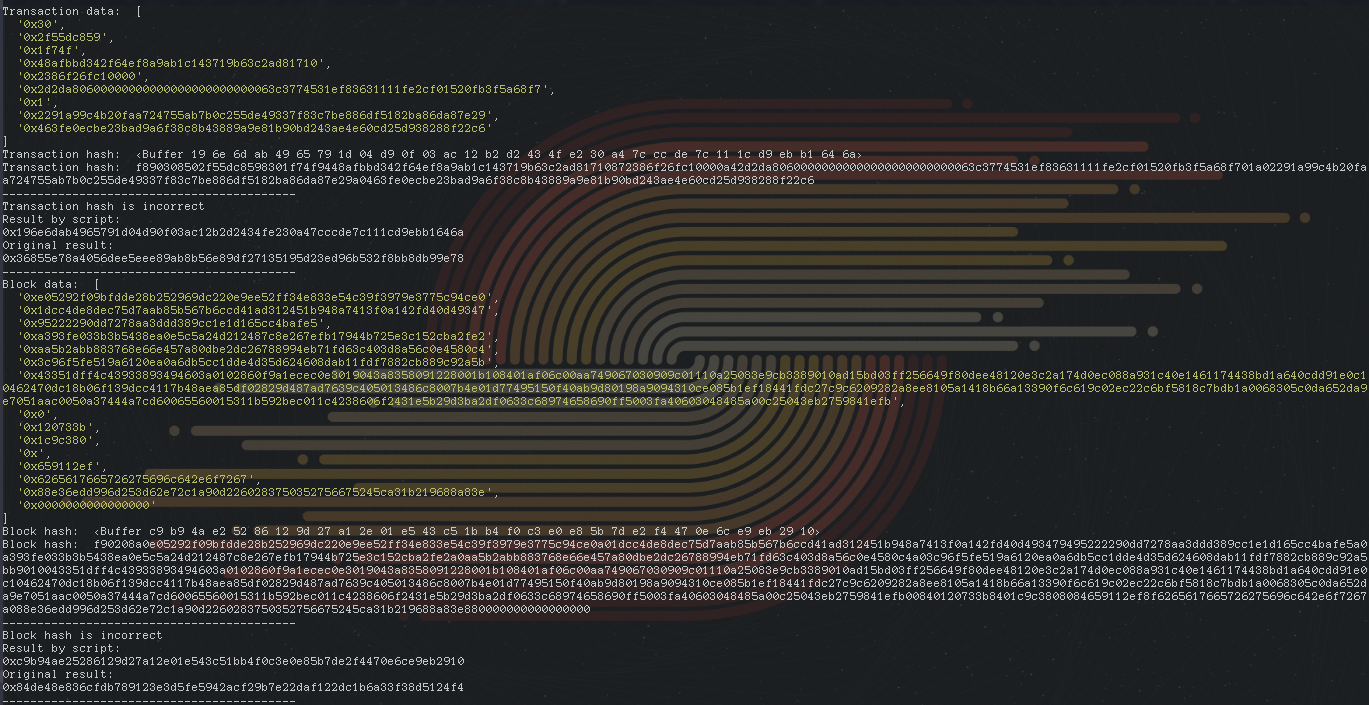
\includegraphics[width=1\linewidth]{img/HashPostMergeError}
	\caption{Output of the hashing process using post-merge data with the same process}
	\label{fig:hashpostmergeerror}
\end{figure}

This improper output happens because the data post-merge change so the hashing method has a different input \cite{eth_MergeAnswer_2023} further investigation about how transaction and block hashing is made post-merge is required to get a correct output. 

All scripts can be find in \url{https://github.com/Roll-a-Mate/Research/tree/main/0002-Strengthening%20Cryptobridges/code}


\newpage
\bibliography{citations}

\end{document}